\documentclass{article}
\usepackage{graphicx}
\usepackage{siunitx}
\graphicspath{ {images/} }
\title{Refrigerator Sliding Down Ramp}
\author{Grant Curell}
\begin{document}
\maketitle{}
\section{Previous Problem}
I didn't do this one, but the information is relevant.

What if you have to drag a heavy object up a ramp? Say, for example, you have to move a refrigerator. You want to go camping, and because you expect to catch plenty of fish, you decide to take your 100-kilogram refrigerator with you. The only catch is getting the refrigerator into your vehicle (see Figure 6-4). The refrigerator has to go up a \ang{30} ramp that happens to have a static coefficient of friction with the refrigerator of 0.20 and a kinetic coefficient of friction of 0.15 (see the earlier section "On the move: Understanding static and kinetic friction"). The good news is that you have two friends to help you move the fridge. The bad news is that you can supply only 350 newtons of force each, so your friends panic.
\\\\
Holzner, Steven. Physics I For Dummies (For Dummies (Math \& Science)) (p. 108). Wiley. Kindle Edition.

\section{Problem}
Assuming that the ramp and the ground both have the same kinetic coefficient of friction and that the refrigerator starts to slide from the top of the ramp, how far will the refrigerator that your friends drop (in the preceding section) slide? Take a look at Figure 6-5, which shows the refrigerator as it slides down the 3.0-meter ramp. As you watch with dismay, it picks up speed. A car is parked behind the ramp, only 7.2 meters away. Will the errant refrigerator smash it?

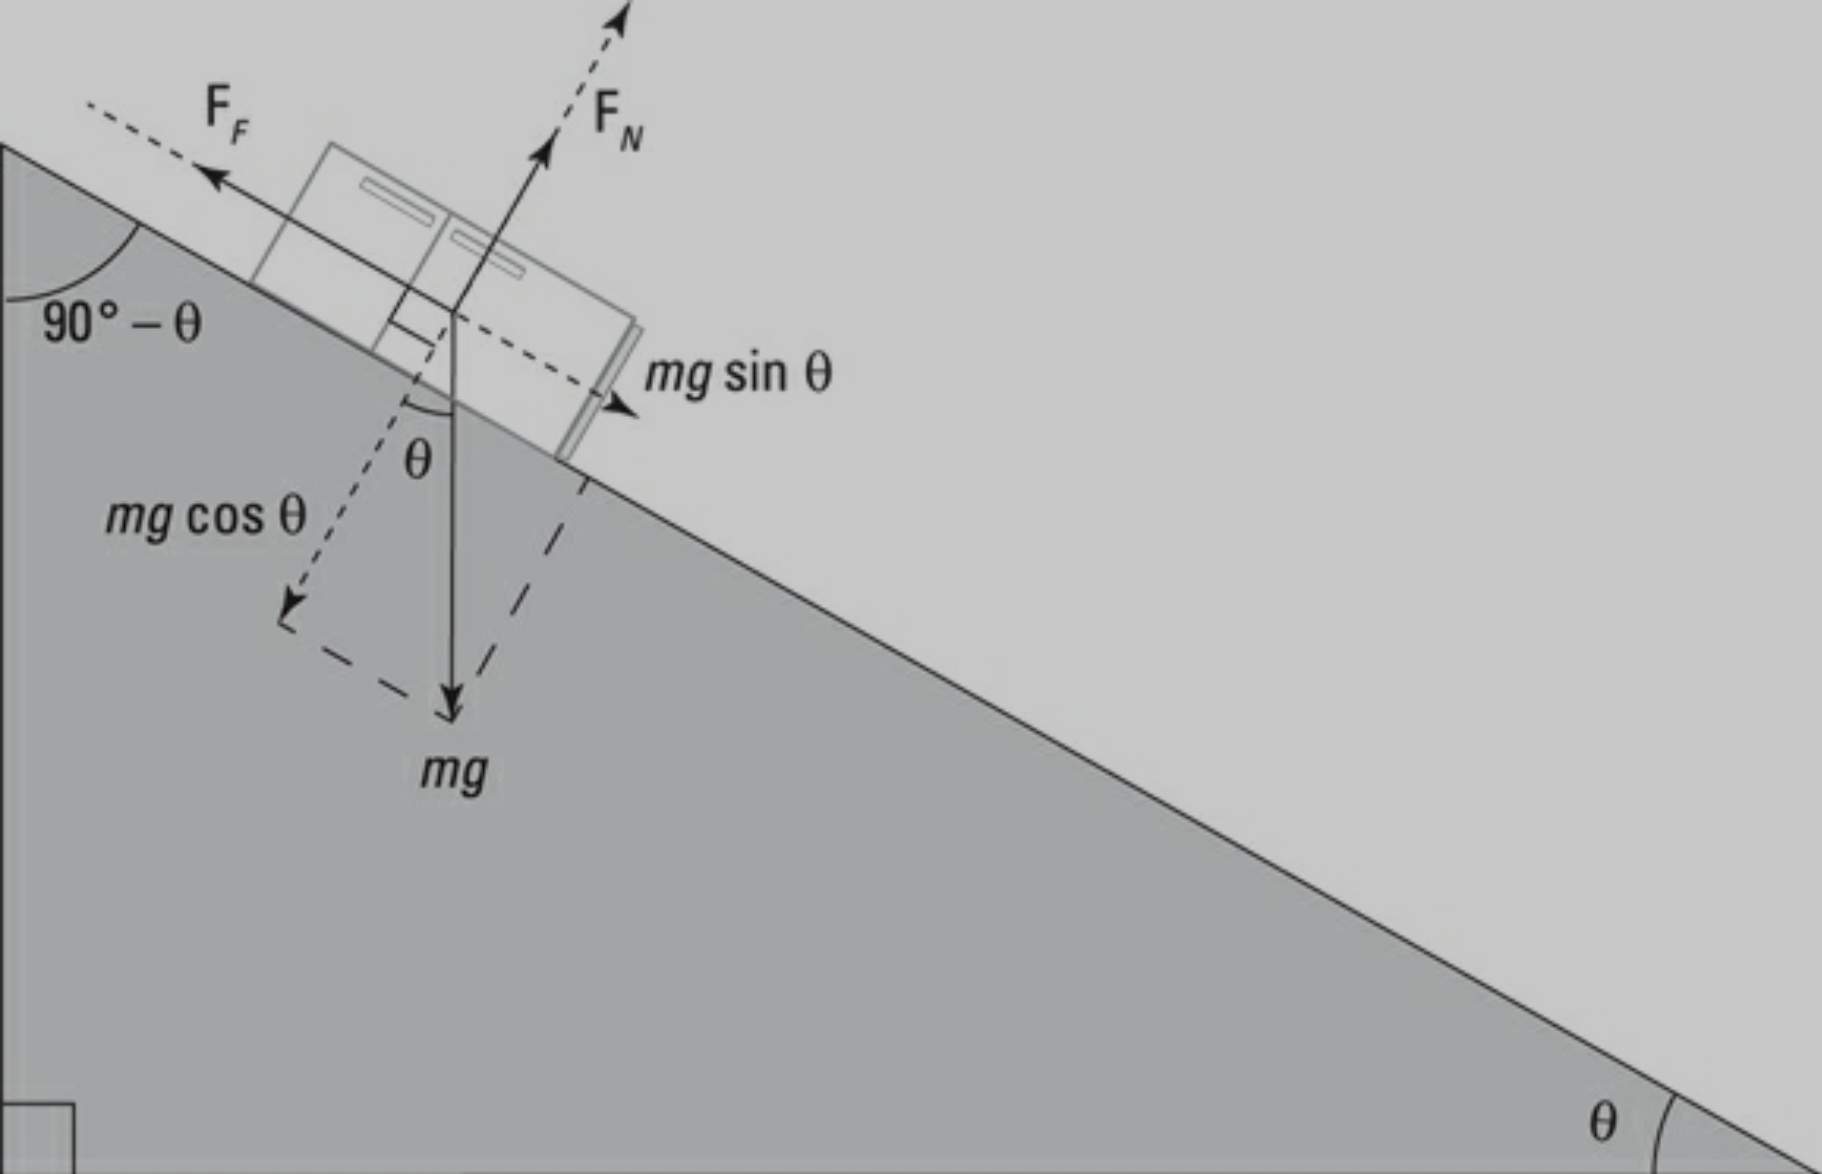
\includegraphics[width=\columnwidth]{image}
\\\\
Holzner, Steven. Physics I For Dummies (For Dummies (Math \& Science)) (pp. 110-111). Wiley. Kindle Edition.
\\\\
\section{Solution}
\[ \mu_k = .15 \]
\[ s_{ramp}=3m \]
\[ m_{fridge}=100kg \]
\[ F_{normal}=mg\cos(30) \]
\[ F_{kinetic}=.15(mg\cos(30)) \]
\[ F_{total}=mg\sin(30)-.15(mg\cos(30)) \]
\[ a_{fridge}=g\sin(30)-.15g\cos(30) \]
I will assume that the ground has the same coefficient of friction as does the ramp.
\[  v_f=v_i+at \]
\[ s=v_it+\frac{1}{2}at^2 \]
\[ 3=0*t+\frac{at^2}{2} \]
\[ t=1.29s \]
It takes 1.29s for the refrigerator to reach the bottom of the ramp. Since our acceleration is 3.63 our exit velocite is \[ 3.63*1.29 \] which is \[ 4.68m/s \]
\[ F_{friction}=.15(100)9.8=147N \]
\[ -147=100a \]
\[ -1.47m/s^2=a_{fridge} \]
\[ a=\frac{\triangle{v}}{\triangle{t}} \]
\[ t=3.18s \]
It takes 3.18 seconds for the fridge to stop.
\[ s=\bar{v}t \]
\[ \bar{v} = \frac{v_i+v_f}{2} \]
\[ s=\frac{4.68}{2}*3.18 \]
\[ s=7.44m \]
It won't be by much, but I conclude the fridge will hit the car (which was 7.2m away).
\section{Question}
I haven't investigated why, but the book came to the conclusion of 7.1 meters. That's close enough and glancing at the way they did it they probably rounded differently. I'm guessing I rounded incorrectly because they came to the conclusion that the refrigerator narrowly stops before hitting the car.
\end{document}
